% Chapter 4

\chapter{Results} % Main chapter title

\label{Chapter4}  

\section{Artefact}
The artefact that was developed is a computer game and is titled \textit{"Puzzle Ball: Spherical Shadows"} and is a self-contained application that can be launched standalone without any additional software needed. While it is fairly lightweight on hardware resources for a computer game, it does require more resources than a typical application and may stutter on older systems due to the effects used. In terms of the genres it encompass, it would full under the platformer, puzzle and action genres for games and as such is described as a 3D puzzle platformer with aspects of action gameplay played in first person.
\\\\
Once the application is launched, the user is taken to the \textit{Main Menu} screen (depicted below) where clicking the text \textit{Play} triggers a function to start the first level - that being the the Tutorial. Each group member was responsible for the design of an individual level where the Tutorial/First level being the level undertaken in this project. The reason for this is that the research aspect of this project aligns with the goals of a tutorial level. 

\begin{figure}[H]
\centering
\begin{subfigure}{0.5\textwidth}
  \centering
  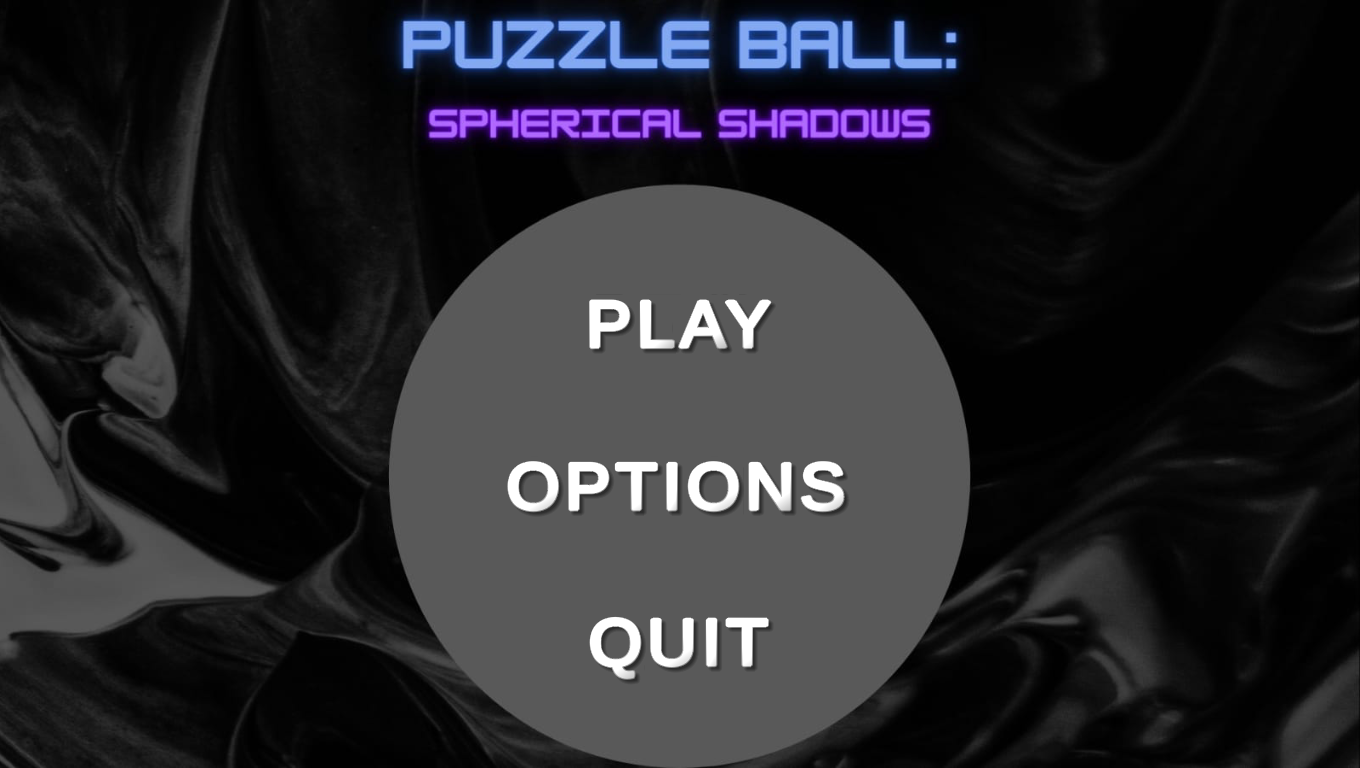
\includegraphics[width=1\linewidth]{Figures/menu.png}
  \caption{The Main Menu of the Artefact}
\end{subfigure}%
\begin{subfigure}{0.5\textwidth}
  \centering
  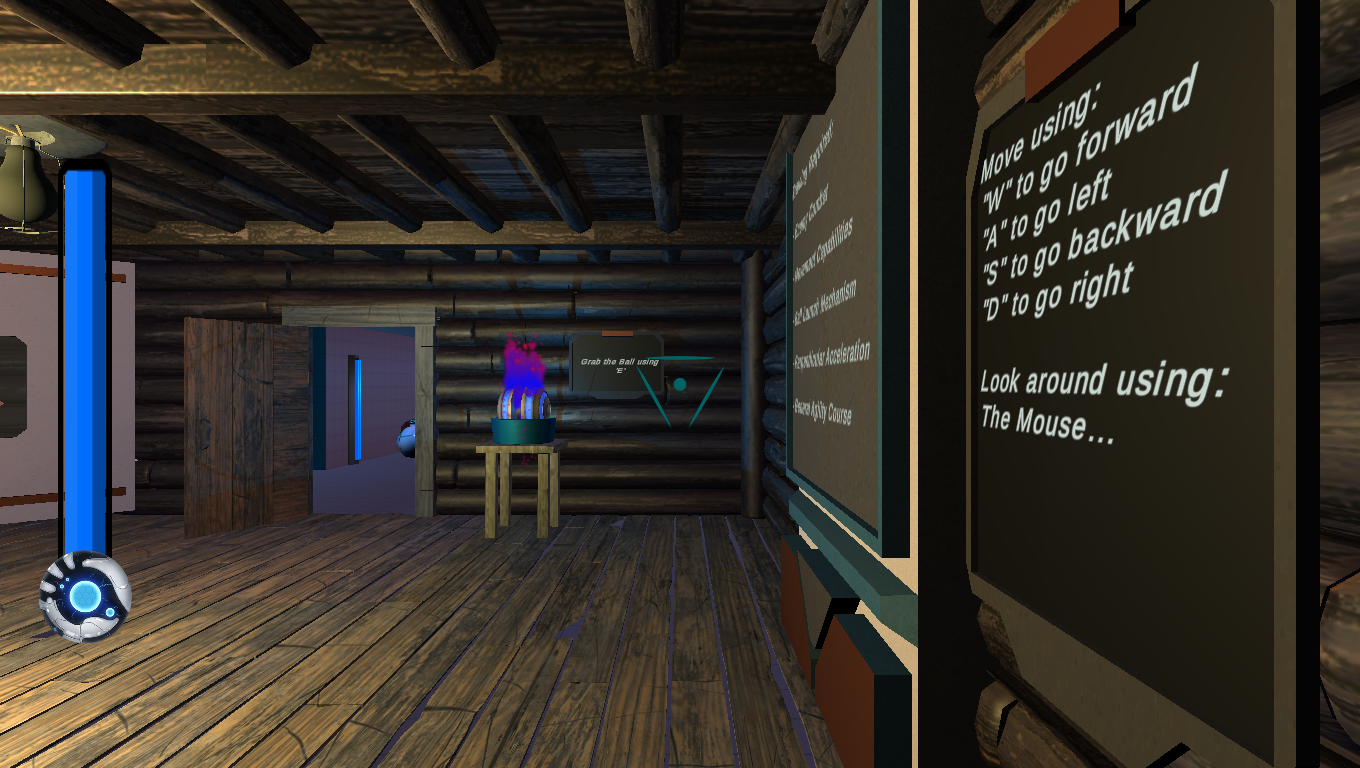
\includegraphics[width=1\linewidth]{Figures/start.png}
  \caption{The Starting Point of the Level}
\end{subfigure}
\caption{Starting the Game}
\end{figure}

\noindent One the tutorial level has started, the user is shown the basic character movement controls on the right side of the screen and can continue forward. Text based signs were used throughout the level to explain various mechanics or tasks to be completed - an example of this is shown in Figure 4.2 below.

\begin{figure}[H]
\centering
\centerline{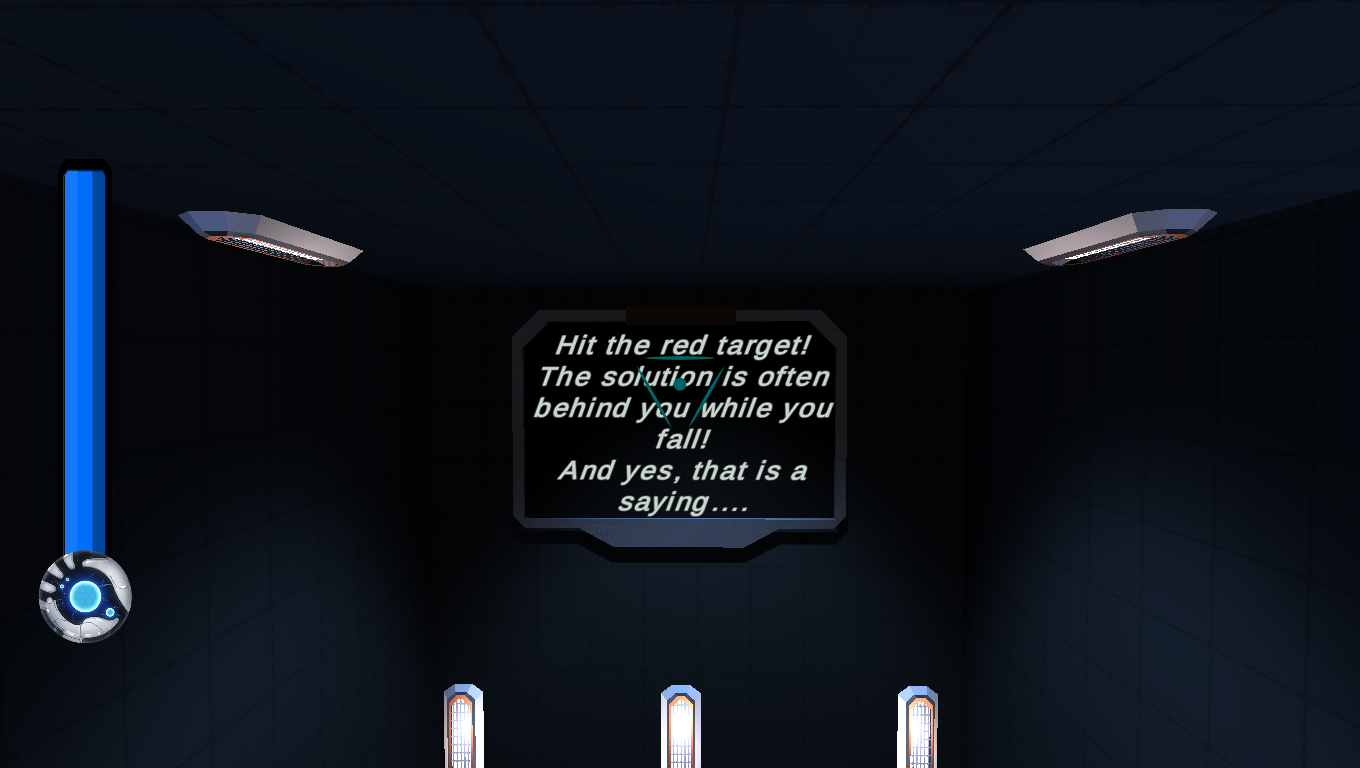
\includegraphics[scale=0.33]{tutSignEg.png}}
\caption{A Further Example of the Tutorial Signs}
\end{figure}

\noindent The user must then make there way to a central area, referred to as the Hub Room, where they are given the choice in what order they would like to complete the five main tutorials. These will be discussed and shown below. As the user completes the several tutorials, a blockade that restricted movement to the next level is slowly removed as shown below.

\begin{figure}[H]
\centering
\begin{subfigure}{0.3\textwidth}
  \centering
  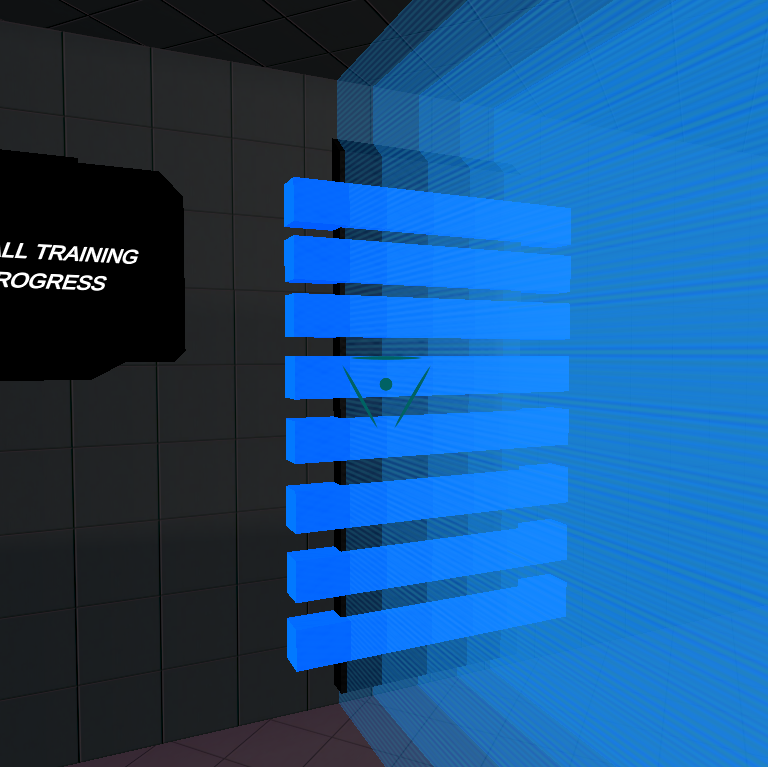
\includegraphics[width=1\linewidth]{Figures/barrier5.png}
  \caption{No Tutorials Completed}
\end{subfigure}%
\begin{subfigure}{0.3\textwidth}
  \centering
  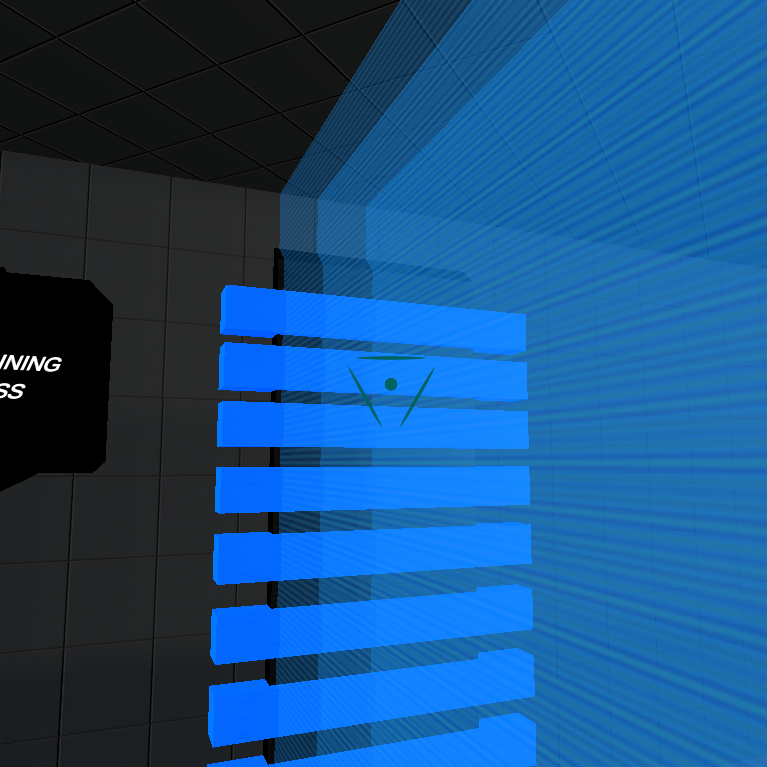
\includegraphics[width=1\linewidth]{Figures/barrier3.png}
  \caption{Two Tutorials Completed}
\end{subfigure}
\begin{subfigure}{0.3\textwidth}
  \centering
  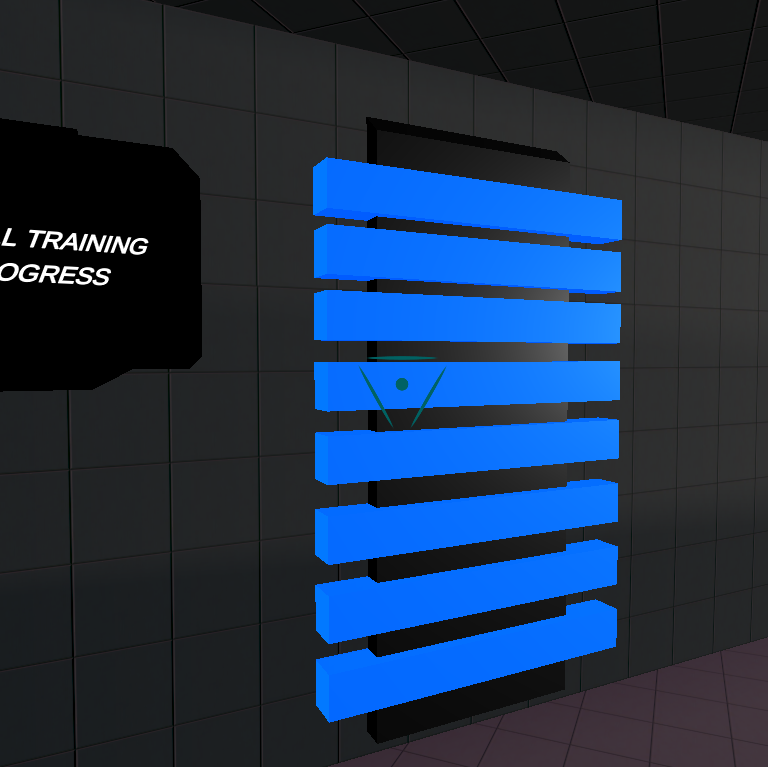
\includegraphics[width=1\linewidth]{Figures/barrier0.png}
  \caption{All Tutorials Completed}
\end{subfigure}
\caption{Progress Blocker in Tutorial}
\end{figure}

\noindent Once all the tutorials in this level are completed and the blockade removed, the user is allowed to move towards the final room where they must throw the ball object into the centre of the desk-like object with a particle effect on it.

\begin{figure}[H]
\centering
\centerline{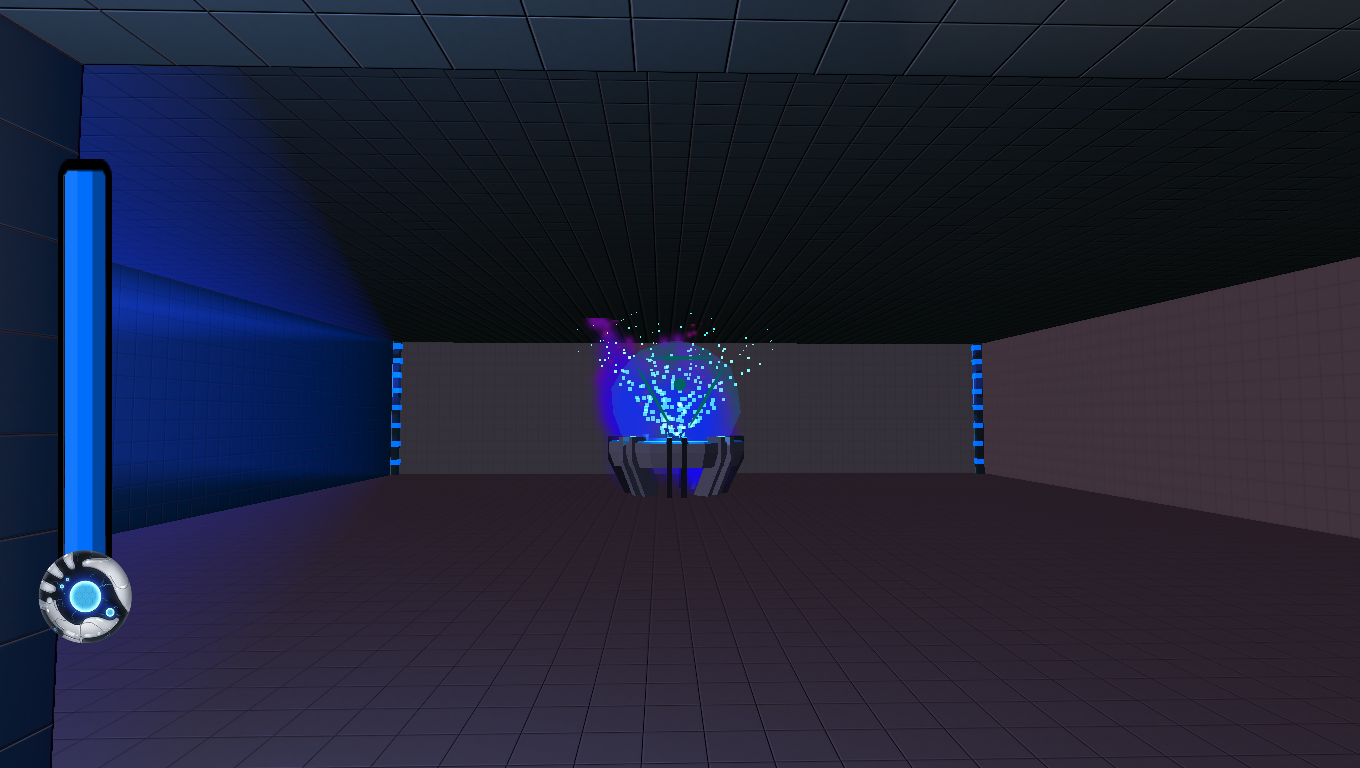
\includegraphics[scale=0.33]{Figures/endgoal.png}}
\caption{The End Goal Object}
\end{figure}

\noindent Once the ball object collides with the end goal object, the user is taken to the next level where the main aim to to traverse the level and throw the ball object into the next end goal. This process is followed for two additional levels for three in total  after which the user is taken to a scene where the group members and their contributions are listed with a prompt to close the application.

\begin{figure}[H]
\centering
\centerline{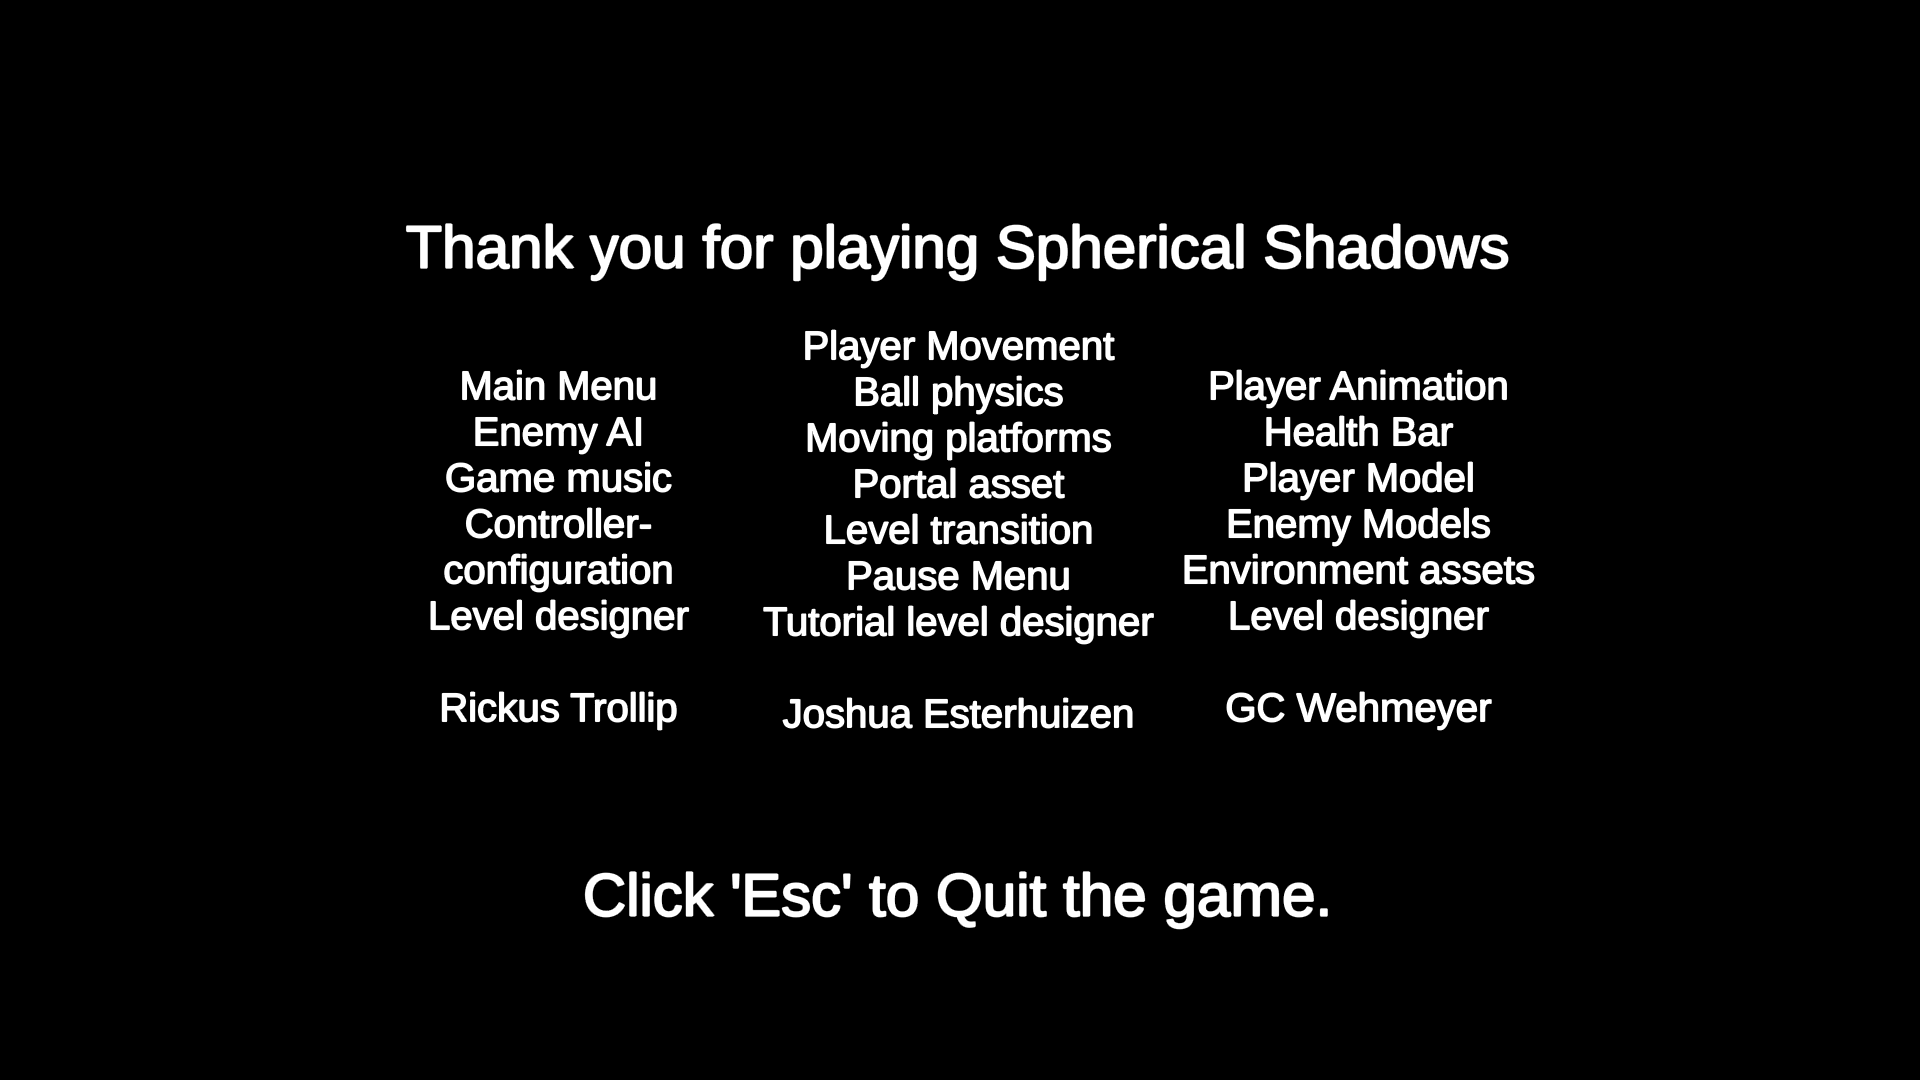
\includegraphics[scale=0.33]{Figures/credits.png}}
\caption{The Credits Screen}
\end{figure}

\section{Article}
A literary analysis on the fields of pedagogy, ludology and gamification was conducted and an article written in order to answer the question posed; \textit{What qualities and principles can be applied to a video game to allow it to be used in a learning environment as a means to provide better engagement among certain students by providing an enjoyable delivery of information?}
\\\\
This question was then refined and phrased as \textit{What qualities are required for a serious game to be effectively used in an educational environment on various topics?} within the article.
\\\\
The results of the research aspect of this project is the answer to these questions which were synthesised from various case studies and the literature analysis conducted.

\section{Conclusion}